%%%%%%%%%%%%%%%%%%%%%%%%%%%%%%%%%%%%%%%%%%%%%%%%%%%%%%%
%% Engineer & Master Thesis, LaTeX Template          %%
%% Copyleft by Piotr Woźniak & Artur M. Brodzki      %%
%% Faculty of Electronics and Information Technology %%
%% Warsaw University of Technology, Warsaw, 2019     %%
%%%%%%%%%%%%%%%%%%%%%%%%%%%%%%%%%%%%%%%%%%%%%%%%%%%%%%%

\documentclass[
    left=2.5cm,         % Sadly, generic margin parameter
    right=2.5cm,        % doesnt't work, as it is
    top=2.5cm,          % superseded by more specific
    bottom=3cm,         % left...bottom parameters.
    bindingoffset=6mm,  % Optional binding offset.
    nohyphenation=true % You may turn off hyphenation, if don't like. =false
]{eiti/eiti-thesis} % bazuje na clasie mwart


\usepackage[
    backend=bibtex,
    style=ieee
]{biblatex}
\usepackage{csquotes}
\usepackage{hyperref}

\langpol % Dla języka angielskiego mamy \langeng
\graphicspath{{img/}}             % Katalog z obrazkami.
\addbibresource{bibliografia.bib} % Plik .bib z bibliografią

% dodanie kropki po numerze w~LoL https://tex.stackexchange.com/questions/597350/add-dot-after-number-of-listing-in-list-of-listings
\makeatletter
\xpatchcmd\lst@MakeCaption{\protect\numberline{\thelstlisting}\lst@@caption}{\protect\numberline{\thelstlisting.}\lst@@caption}{}{}
%\makeatother
%\makeatletter
%\xpatchcmd{\LT@c@ption}{\protect\numberline{\thetable}}{\protect\numberline.{. \thetable . }}{}{}
\makeatother

\begin{document}

%--------------------------------------
% Strona tytułowa
%--------------------------------------
%\MasterThesis % dla pracy inżynierskiej mamy 
\RaportThesis
\instytut{Cyberbezpieczeństwa}
\kierunek{Telekomunikacja}
\specjalnosc{Techniki Teleinformatyczne}
\title{
    Akceleracja sprzętowa kryptoanalizy algorytmów kryptograficznych
}
\engtitle{ % Tytuł po angielsku do angielskiego streszczenia
    Hardware acceleration of cryptoanalysis of cryptograhpic algorithms
}
\author{Andrzej Tłomak}
\album{311450}
\promotor{dr. hab. inż. Mariusz Rawski}
\date{\the\year}
\maketitle

%--------------------------------------
% Streszczenie po polsku
%--------------------------------------
%\streszczenie
%Celem tego etapu było zapoznanie się z literaturą opisującą aktualny \
%State~of~the~Art kryptoanalizy systemów opartych o krzywe eliptyczne w ciałach skończonych, \
%zapoznanie się z teorią oraz podstawami matematycznymi zagadnienie krzywych eliptycznych w \
%kryptografii oraz przygotowanie środowiska do pracy z wykorzystaniem technologii CUDA. \
%\slowakluczowe Krzywe eliptyczne, Kryptografia, Kryptoanaliza, CUDA, FPGA, Algorytm~rho~Pollard'a
%
%\newpage
%
%%--------------------------------------
%% Streszczenie po angielsku
%%--------------------------------------
%\abstract
%The objective of this phase included a review of the literature describing the current State-of-Art \
%in cryptoanalysis of systems \
%based on Elliptic curves in Finite Fields. It involved getting deeper knowledge of theory
%and mathematical fundation of Elliptic curves as well as setting up an environment
%to develop implementation utillizing CUDA technology.
%\keywords Elliptic curves, Cryptography, Cryptoanalysis, CUDA, FPGA, rho~Pollard~algorithm
%\newpage

%--------------------------------------
% Oświadczenie o autorstwie
%--------------------------------------
%\makeauthorship
%\blankpage

%--------------------------------------
% Spis treści
%--------------------------------------
%\thispagestyle{empty}
\tableofcontents
%\blankpage

%--------------------------------------
% Rozdziały
%--------------------------------------
\newpage % Zaleca się otwieranie rozdziału od nowej strony.
\section{Plan na semestr 2023Z}
Celem tego etapu było zapoznanie się z literaturą opisującą aktualny \
State~of~the~Art kryptoanalizy systemów opartych o krzywe eliptyczne w ciałach skończonych, \
zapoznanie się z teorią oraz podstawami matematycznymi zagadnienie krzywych eliptycznych w \
kryptografii oraz przygotowanie środowiska do pracy z wykorzystaniem technologii CUDA. \
\newline

\indent
Status zaplanowanych zadań:
\begin{itemize}
    \item \hyperref[sc:state]{Przegląd literatury} - \textbf{zrealizowane}
    \item \hyperref[sc:wstep]{Zapoznanie się z podstawami matematycznymi}-
    \textbf{zrealizowane}
    \item Konfiguracja środowiska pracy (CUDA oraz SageMath) - \textbf{zrealizowane}
    \item Implementacja i testowanie prototypu w technologii CUDA - \textbf{w trakcie}
\end{itemize}

\newpage % Zaleca się otwieranie rozdziału od nowej strony.
\section{Wstęp teoretyczny}
\label{sc:wstep}
W tym etapie jednym z zaplanowanych celów, było zapoznanie się z teorią stojącą za
kryptografią krzywych eliptycznych. Aby jednak zrozumieć to zagadnienie, musiałem również
zgłębić szersze pole tej dziedziny kryptografii, jaką jest kryptografia oparta o \textbf{problem logarytmu dyskretnego}, zarówno na krzywych eliptycznych jak i innych, odpowiednich grupach.
\newline

\indent
Każde wymienione poniżej zagadnienie, zaimplementowałem również w pakiecie obliczeniowym SageMath. Odpowiadające zaganieniom listingi kodu znajdują się w dalszej części raportu.
\subsection{Problem logarytmu dyskretnego}
Problem logarytmu dyskretnego (\textbf{DLP}) jest podstawą wielu kryptosystemów. Najbardziej znanym z nich jest kryptosystem ElGamala. Problem logarytmu dyskretnego
można przedstawić zarówno na grupie multiplikatywnej $(\mathbb{G},\cdot)$
oraz grupie addytywnej, przy odpowiednim zdefiniowaniu
operacji dodawania na krzywej eliptycznej $(\mathbb{E},+)$ \cite{stinson21}.

\subsection{DLP w grupie multiplikatywnej}
Jeżeli $\mathbb{G}$ to (skończona) grupa multiplikatywna, $\alpha \in \mathbb{G}$
to element rzędu $n$ oraz $\beta \in \mathbb{<\alpha>}$ (jest w podgrupie generowanej
przez $\alpha$), to uważane za problematyczne jest znalezienie takiej liczby $a$:
\[a \in \mathbb{Z} \textrm{ oraz } 0\le a \le n-1\]
że:
\[\alpha ^ a = \beta\]

Liczbę $a$ można przedstawić jako:
\[\log_{\alpha}{\beta}\]


\subsection{DLP w grupie addytywnej}
W przypadku krypografii opartej o krzywe eliptyczne, DLP dotyczy
grupy addytywnej $(\mathbb{E},+)$ zdefiniowanej na krzywej eliptycznej.
Niech $\alpha$ jest rzędu n.
W takim przypadku, ponieważ operacją na grupie jest dodawanie modulo n, to działanie
potęgowania przedstawia się jako:
\[\alpha \cdot a = \beta \textrm{ (mod } n)\]
Przy odpowiednim wyborze grupy addytywnej, rozwiązanie problemu logarytmu dyskretnego,
tj. znalezienie $a$,
jest trudne \cite{chrzaszczyk2010}\cite{stinson21}.
\subsection{Krzywe eliptyczne}
Krzywą eliptyczną nieosobliwą nad ciałem $\mathbb{K}$ o charakterystyce różnej od 2 i 3 definiuje się
za jako zbiór rozwiązań $(x,y) \in \mathbb{R} \times \mathbb{R}$ równiania: \cite*{stinson21}
\[y^2 = x^3 + ax + b\]
przy założeniu, że stałe $a, b$ takie, że:
\[4a^3 + 27b^2 \not= 0\]
Jest to tak zwana forma {\it Weierstrassa} krzywej eliptycznej.

\subsubsection{Krzywe eliptyczne na liczbach rzeczywistych}

Krzywe eliptyczne zdefiniowane na liczbach rzeczywistych nie są kluczowe w
systemach kryptograficznych\cite*{chrzaszczyk2010}\cite*{stinson21}, ale takie ustawienia
pozwalają na prostsze przedstawienie niektórych zagadnień
np. dodawnie punktów na krzywej.
\begin{figure}[!h]
    \centering 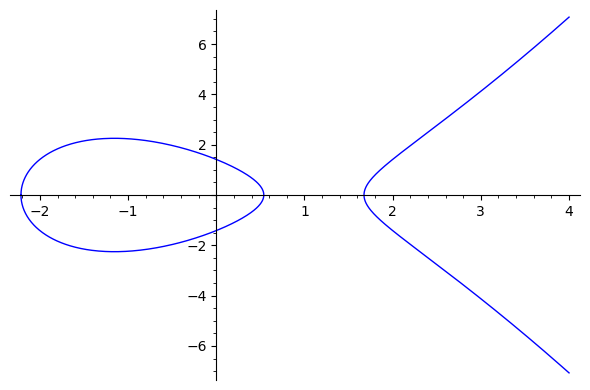
\includegraphics[width=0.8\linewidth]{sage/krzywa_-4_2.png}
    \caption{Krzywa eliptyczna $y^2=x^3-4+2$}
\end{figure}

\subsubsection*{Krzywe eliptyczne na ciele skończonym}
Krzywa eliptyczna na ciele skończonym jest stosowana w kryptografii.
Z powodu charakterystyki ciała, jej wykres
nie przypomina krzywej na liczbach rzeczywistych.
Krzywa taka składa się z punktów, których współrzędne należą do ciała
na którym jest opisana.
Wszystkie operacje na krzywej, takie jak dodawanie, wykonuje się
również z zastosowaniem operacji modulo rzędu ciała.
\begin{figure}[!h]
    \centering 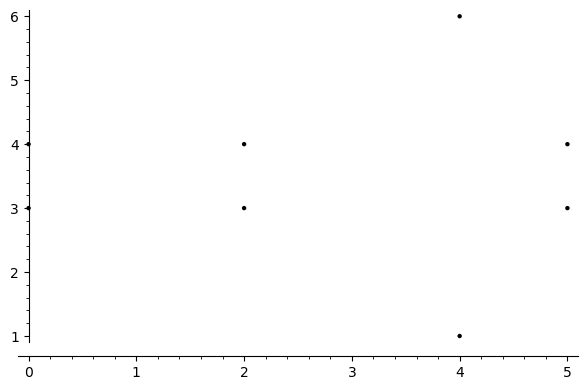
\includegraphics[width=0.8\linewidth]{sage/elliptic_finite_field.png}
    \caption{Krzywa eliptyczna $y^2=x^3-4+2$ nad $GF(7)$}
\end{figure}

\subsubsection{Dodawanie punktów na krzywej eliptycznej}
Przedstwienie krzywej eliptycznej na ciele liczb rzeczywistych,
umożliwia proste zwizualizowanie geometrycznej interpretacji dodawania punktów
leżących na krzywej.
\newline
\indent
Geometryczne dodawanie punktów na krzywej eliptycznej polega na połączeniu
dwóch punktów $P$ i $Q$ prostopadłą linią, która przecina krzywą w trzecim
punkcie, $R'$. Następnie, wynikowy punkt $R$, będący sumą $P+QP+Q$, znajdujemy przez
odbicie punktu $R'$ względem osi $x$. W przypadku dublowania punktu, czyli dodawania
punktu PP do siebie samego, rysujemy styczną do krzywej w punkcie $P$, która przecina
krzywą w nowym punkcie. Odbicie tego punktu względem osi $x$ daje nam wynik $2P$.
\newline
Kod w SageMath użyty do wizualizacji dodawania: listing \ref*{sage_1}
\begin{figure}[!h]
    \centering 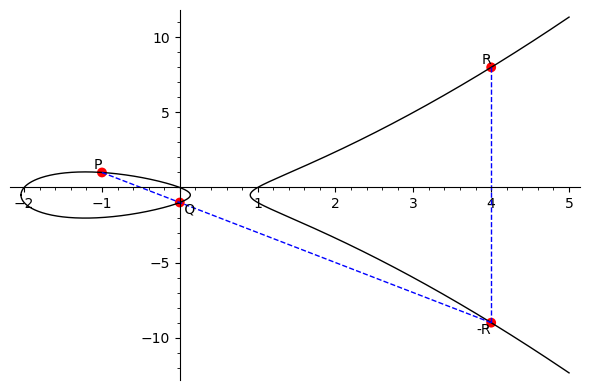
\includegraphics[width=0.8\linewidth]{sage/elliptic_rational_point_addition.png}
    \caption{P + Q na krzywej eliptycznej $y^2+y=x^3-x^2+2x$}
\end{figure}
\newpage

\subsubsection{Dodawanie punktów na krzywej zdefiniowanej na ciele skończonym}
Dodawanie punktów krzywej eliptycznej na ciele skończonym nie ma przejrzyjstej
reprezentacji geometrycznej.
W tym celu stosuje się podejście analityczne.
Wtedy, dodawanie wygląda w następujący sposób:
\begin{enumerate}
    \item Przypadek, gdy \( P \neq Q \):
          \begin{align*}
              \lambda & = \frac{y_2 - y_1}{x_2 - x_1}, \\
              x_3     & = \lambda^2 - x_1 - x_2,       \\
              y_3     & = \lambda(x_1 - x_3) - y_1
          \end{align*}

    \item Przypadek, gdy \( P = Q \):
          \begin{align*}
              \lambda & = \frac{3x_1^2 + a}{2y_1}, \\
              x_3     & = \lambda^2 - 2x_1,        \\
              y_3     & = \lambda(x_1 - x_3) - y_1
          \end{align*}
\end{enumerate}
Dodawanie punktów w SageMath listing \ref{sage_1}

         % W długich pracach
\newpage % Zaleca się otwieranie rozdziału od nowej strony.
\section{State~of~Art}
\label{sc:state}

\subsection{GPU}
Procesory graficzne są dedykowane do wykonywania wielu równoległych obliczeń.
Dzięki temu, są bardzo wydajne w zadaniach które można łatwo zrónoleglić.
Wiele algorytmów do kryptoanalizy pozwala na przetwarzanie równoległe, 
w szczególności algorytm \textbf{rho-Pollarda}.
\subsubsection*{Solving Discrete Logarithms in Smooth-Order Groups with CUDA}
W roku 2012 na karcie graficznej NVIDIA Tesla M2050 osiągnięto wydajność na poziomie
51.9 miliona operacji mnożenia modularnego 768-bit na sekundę.
Implementacja opierała się głównie na języku C z CUDA framework wraz z jednostkowymi segmentami
w języku PTX który jest zbiorem instrukcji dla CUDA GPU.
Praca ma dla mnie szczególną na tym etapie, ponieważ razem z pracą udostępniono kod
implementacji na prawach open-source, dodatkowo opisuje
ograniczenia i założenia jakie należy uwzględnić przy implementacji
algorytmu rho-Pollarda na GPU\cite{henry-goldberg-cuda}.

\subsubsection*{ECC2K-130 on NVIDIA GPUs}
Artykuł opisuje implementację algorytmu rho-Pollarda na karcie graficznej NVIDIA 
GTX 295.
Autorzy wybrali krzywą Koblitza ECC2K-130.
Opisano decyzje związane z wyborem bazy ( w tym przypadku wybrano bazę normalną).
Przedstawiono również szczegóły związane z zarządzaniem pamięcią oraz problem związany
z DRAM'em karty (przy pełnej utylizacji GPU w pamięci brakowało miejsca na input)
Wynik: Średnio obliczenie ECDLP na tej krzywej zajełoby 2 lata przy 534 kartach.

\subsection{FPGA}
\subsubsection*{Solving Discrete Logarithms in Smooth-Order Groups with CUDA}
W 2014 opublikowano pracę przedstawiającą implementację FPGA
na platformie Virtex-6.
dedykowaną do rozwiązania logarytmu dyskretnego na 113-bitowej krzywej Koblitza.
Opisano zastosowane zabiegi poprawiające optymalizację, oraz design
poszczególnych moduł
Na przykład w celu lepszej optymalizacji, wykorzystano bazę normalną
$F_{2^m}$ w jednym z modułów do liczenia automorfizmu punktów.
Wynik po ekstrapolacji to 28 dni na rozwiązanie logarytmu na krzywej Koblitza 113 bit.

\subsection{CPU}
CPU nie są najwydajniejszą architekturą do wykonywania równoległych obliczeń.
Zazwyczaj charakteryzują się znacznie wydajniejszymi jednostkami obliczeniowymi (rdzeniami)
niż na przykład GPGPU, ale jest ich również znacznie mnniej niż w GPGPU.
CPUs są najlepiej przystosowane do przetwarzania potokowego.
\subsubsection*{A Review on solving ECDLP over Large Finite Field using Parallel
	Pollard's Rho (p) Method}
Praca przedstawia wyniki czasowe przy obliczaniu ECDLP na
ciele skończonym rzędu p do 85-bitów.
Zastosowano do tego cluster CPU o 256 rdzeniach octa-core.
Artykuł również jest interesujący ponieważ zwięźle opsuje background matematyczny
oraz przejrzyście przedstawia wersję równoległą
algorytmu rho Pollarda\cite{rewiev-elliptic-cpu}.
Wynik to 52 godziny dla krzywej na ciele rozmiaru p = 85-bitów.


    % wygodnie jest trzymać
\newpage % Zaleca się otwieranie rozdziału od nowej strony.
\section{Code listings}
\subsection*{Dodawnie punktów na krzywej eliptycznej nad $\mathbb{R}$}

\begin{lstlisting}[language=python, label=sage_1, caption=Dodawnie punktów na krzywej eliptycznej na liczbach rzeczywistych]
# SageMath kernel

sage: R = P + Q
sage: R_inv = -R

# Plot elliptic curve
sage: plot_curve = plot(E, rgbcolor="black", xmax=5)

# Plot points
sage: plot_p = plot(P, marker="o", rgbcolor="red", size=50)
sage: p_label = text(
    "P",
    P.dehomogenize(2),
    horizontal_alignment="right",
    vertical_alignment="bottom",
    color="black",
)
sage: plot_q = plot(Q, marker="o", rgbcolor="red", size=50)
sage: q_label = text(
    " Q",
    Q.dehomogenize(2),
    horizontal_alignment="left",
    vertical_alignment="top",
    color="black",
)
sage: plot_r = plot(R, marker="o", rgbcolor="red", size=50)
sage: r_label = text(
    "R",
    R.dehomogenize(2),
    horizontal_alignment="right",
    vertical_alignment="bottom",
    color="black",
)
sage: plot_r_inv = plot(R_inv, marker="o", rgbcolor="red", size=50)
sage: r_inv_label = text(
    "-R",
    R_inv.dehomogenize(2),
    horizontal_alignment="right",
    vertical_alignment="top",
    color="black",
)

sage: p6 = line2d(
    [P.dehomogenize(2), R_inv.dehomogenize(2)], linestyle="--", rgbcolor="blue"
)
sage: p7 = line2d(
    [R.dehomogenize(2), R_inv.dehomogenize(2)], linestyle="--", rgbcolor="blue"
)

sage: plot_curve + plot_p + plot_q + plot_r + plot_r_inv + p6 + p7 + p_label + q_label + r_label + r_inv_label
\end{lstlisting}

\subsection*{Dodawnie punktów na krzywej eliptycznej nad $\mathbb{GF}(7)$}
\begin{lstlisting}[language=python, label=sage_2, caption=Dodawnie punktów na krzywej eliptycznej zdefiniowanej na GF(7)]
Gf = GF(7)

E = EllipticCurve(Gf,[3,4])

def ell_add(E, P1, P2):
    a, b, p = E
    if P1 == "inf": return P2
    if P2 == "inf": return P1
    x1, y1 = P1; x2,y2 = P2
    x1 %= p; y1 %= p; x2 %= p; y2 %= p;

    if x1 == x2 and y1 == p-y2: return "inf"

    if P1 == P2:
        if y1 == 0: return "inf"
        lam = (3*x1^2+a) * inverse_mod(2*y1,p)
    else:
        lam = (y1-y2) * inverse_mod(x1-x2,p)
    x3 = lam^2 - x1 - x2
    y3 = -lam*x3 - y1 + lam*x1
    return (x3%p, y3%p)

P1 = E.random_point()

p1 = (2,5)
print(p1)
for _ in range(9):
    p1 = ell_add(e, p1, p1)
    p1 = (Integer(p1[0]),Integer(p1[1]))
    print(p1)


\end{lstlisting}

\subsection*{Kryptosystem El-Gamala na $(\mathbb{G}, \cdot)$}
\begin{lstlisting}[language=python, label=sage_3, caption=Kryptosystem El-Gamala]
G = Integers(11)

# Bob:

# Private
x = G(3)

## Public
g = G(5)
h = g^x

# Alice:

# Message
m = G(5)

# Private
k = G(8)

# Public
a = g^k
b = (h^k)*m

# Decrypt Bob:
b*(a^(-1))^x
\end{lstlisting}

\subsection*{Kryptosystem El-Gamala na krzywej $y^2 = x^3 + x + 6 \in \mathbb{GF}(11)$ }
\begin{lstlisting}[language=python, label=sage_3, caption=Kryptosystem El-Gamala na krzywej]
Gf = GF(11)
E = EllipticCurve(Gf, [1, 6])

# Alice -> Bob

# Bob private
m = 7

# Bob public
P = E(2, 7)
Q = m * P


def alice_encrypt():
    k = 6  # random secret variable
    x = 9  # message

    kP = k * P
    kQ = k * Q

    secret_hash = safe_hash_function(kQ)

    y1 = kP
    y2 = (x + secret_hash) % 11
    return (y1, y2)


# just mock, should be secure one way hash fucntion
def safe_hash_function(q):
    if q == E(8, 3):
        return 4
    return 3


# Alice sends cypher
cypher = alice_encrypt()


def bob_decrypt(cypher):
    y1 = cypher[0]
    y2 = cypher[1]

    kQ = m * y1  # m * (kP) / but mP = Q so its kQ

    secret_hash = safe_hash_function(kQ)

    plain_message = (y2 - secret_hash) % 11

    return plain_message


bob_decrypt(cypher)
\end{lstlisting}



\subsection*{Algorytm rho-Pollarda dla grupy multiplikatywnej}
\begin{lstlisting}[language=python, label=sage_4, caption=Algorytm rho-Pollarda dla grupy multiplikatywnej]
class Group_parameters:
    def __init__(self, p, n, alpha, beta) -> None:
        self.p = p
        self.n = n
        self.alpha = alpha
        self.beta = beta

class Triple:
    def __init__(self, x, a, b) -> None:
        self.x = x
        self.a = a
        self.b = b
    def __str__(self) -> str:
        return f"x = {self.x}, a = {self.a}, b = {self.b}"


def f(tripe: Triple, group: Group_parameters) -> Triple:
    if tripe.x % 3 == 1:
        x = group.beta * tripe.x % group.p
        a = tripe.a
        b = tripe.b + 1
        return Triple(x, a, b)
    if tripe.x % 3 == 0:
        x = tripe.x ** 2 % group.p
        a = tripe.a * 2
        b = tripe.b * 2
        return Triple(x, a, b)
    else:
        x = group.alpha * tripe.x % group.p
        a = tripe.a + 1
        b = tripe.b
        return Triple(x, a, b)

g = Group_parameters(809, 101, 89, 618)

t1 = f(Triple(1, 0, 0), g)
t2 = f(t1, g)


i = 1
print('%s %s | %s %s' % (i, t1, 2*i, t2))

i = 2
while(t1.x != t2.x):
    t1 = f(t1, g)
    t2 = f(f(t2, g), g)
    print('%s %s | %s %s' % (i, t1, 2*i, t2))
    i=i+1

print(f"Znaleziona kolizja: x: {t1.x}")
\end{lstlisting}

\subsection*{Algorytm rho-Pollarda znajdowania punktów na krzywej eliptycznej}
\begin{lstlisting}[language=python, label=sage_5, caption=Algorytm rho-Pollarda znajdowania punktów na krzywej eliptycznej]
class Group_parameters:
    def __init__(self, p, alpha, beta) -> None:
        self.p = p
        self.alpha = alpha
        self.beta = beta


class Triple:
    def __init__(self, x, a, b) -> None:
        self.x = x  # Point at Elliptic Curve
        self.a = a  # just a number
        self.b = b  # just a number

    def __str__(self) -> str:
        return f"x = {self.x}, a = {self.a}, b = {self.b}"


def f(tripe: Triple, group: Group_parameters) -> Triple:
    #print("Function run")
    #print(f"Input: {tripe}")

    x_of_xpoint = tripe.x[0]
    y_of_xpoint = tripe.x[1]

    p = group.p

    if int(y_of_xpoint) % 3 == 1:
        x = group.beta + tripe.x
        a = tripe.a
        b = tripe.b + 1
        # check 
        if (x != a * g.alpha + b * g.beta):
            pass
            print(f"1 xab: {x} {a} {b}")
        return Triple(x, a, b)
    if int(y_of_xpoint) % 3 == 0:
        x = 2 * tripe.x
        a = (tripe.a * 2)
        b = (tripe.b * 2)
        if (x != a * g.alpha + b * g.beta):
            pass
            print(f"2 xab: {x} {a} {b}")
        return Triple(x, a, b)
    else:
        x = group.alpha + tripe.x
        a = tripe.a + 1
        b = tripe.b
        if (x != a * g.alpha + b * g.beta):
            pass
            print(f"3 xab: {x} {a} {b}")
        return Triple(x, a, b)


def main(g: Group_parameters, t1):
    i = 1

    t2 = f(t1, g)

    print("%s %s | %s %s" % (i, t1, 2 * i, t2))

    i = 2
    while t1.x != t2.x:
        t1 = f(t1, g)
        t2 = f(f(t2, g), g)
        print("%s %s | %s %s" % (i, t1, 2 * i, t2))
        i = i + 1

    print(f"Found:\nt1: {t1}\nt2: {t2}")

    x = -((t2.a - t1.a) / (t1.b - t2.b))

    print(x)
\end{lstlisting} % każdy rozdział w osobnym pliku. 
%\section{Dodatkowe informacje}
Informacje jak pisać pracę dyplomową oraz szablon pracy zostały wzięte ze strony \href{http://www.ii.pw.edu.pl/ii_pol/Instytut-Informatyki/Nauczanie/Poradnik-dyplomanta/Przygotowanie-pracy-dyplomowej}{http://www.ii.pw.edu.pl/}.

Jak wygląda proces dyplomowania w~IT można dowiedzieć się na stronie \href{https://secure.tele.pw.edu.pl/wp-content/uploads/2017/06/PROCES-DYPLOMOWANIA-17L.pdf}{https:// secure.tele.pw.edu.pl/} w~sekcji Dydaktyka > Dla studentów > Proces dyplomowania.

Aby zacytować artykuł z~Wikipedii, w~łatwy sposób można uzupełnić bibliografię o~tę pozycję. Na stronie z~wybranym artykułem np. o~\href{https://pl.wikipedia.org/wiki/LaTeX}{Latex} ależy po lewej stronie  wybrać 
\textit{Narzędzia:Cytowanie tego artykułu} i~otrzymamy gotowy 
 \href{https://pl.wikipedia.org/w/index.php?title=Specjalna:Cytuj&page=LaTeX&id=58147357}{Przypis do tej strony} \cite{Wiki:Latex}. Na innych stronach należy szukać \textit{bibtex}, \textit{cite} lub podobne.

\subsection{Rysunki}
\begin{figure}[h]
\centering
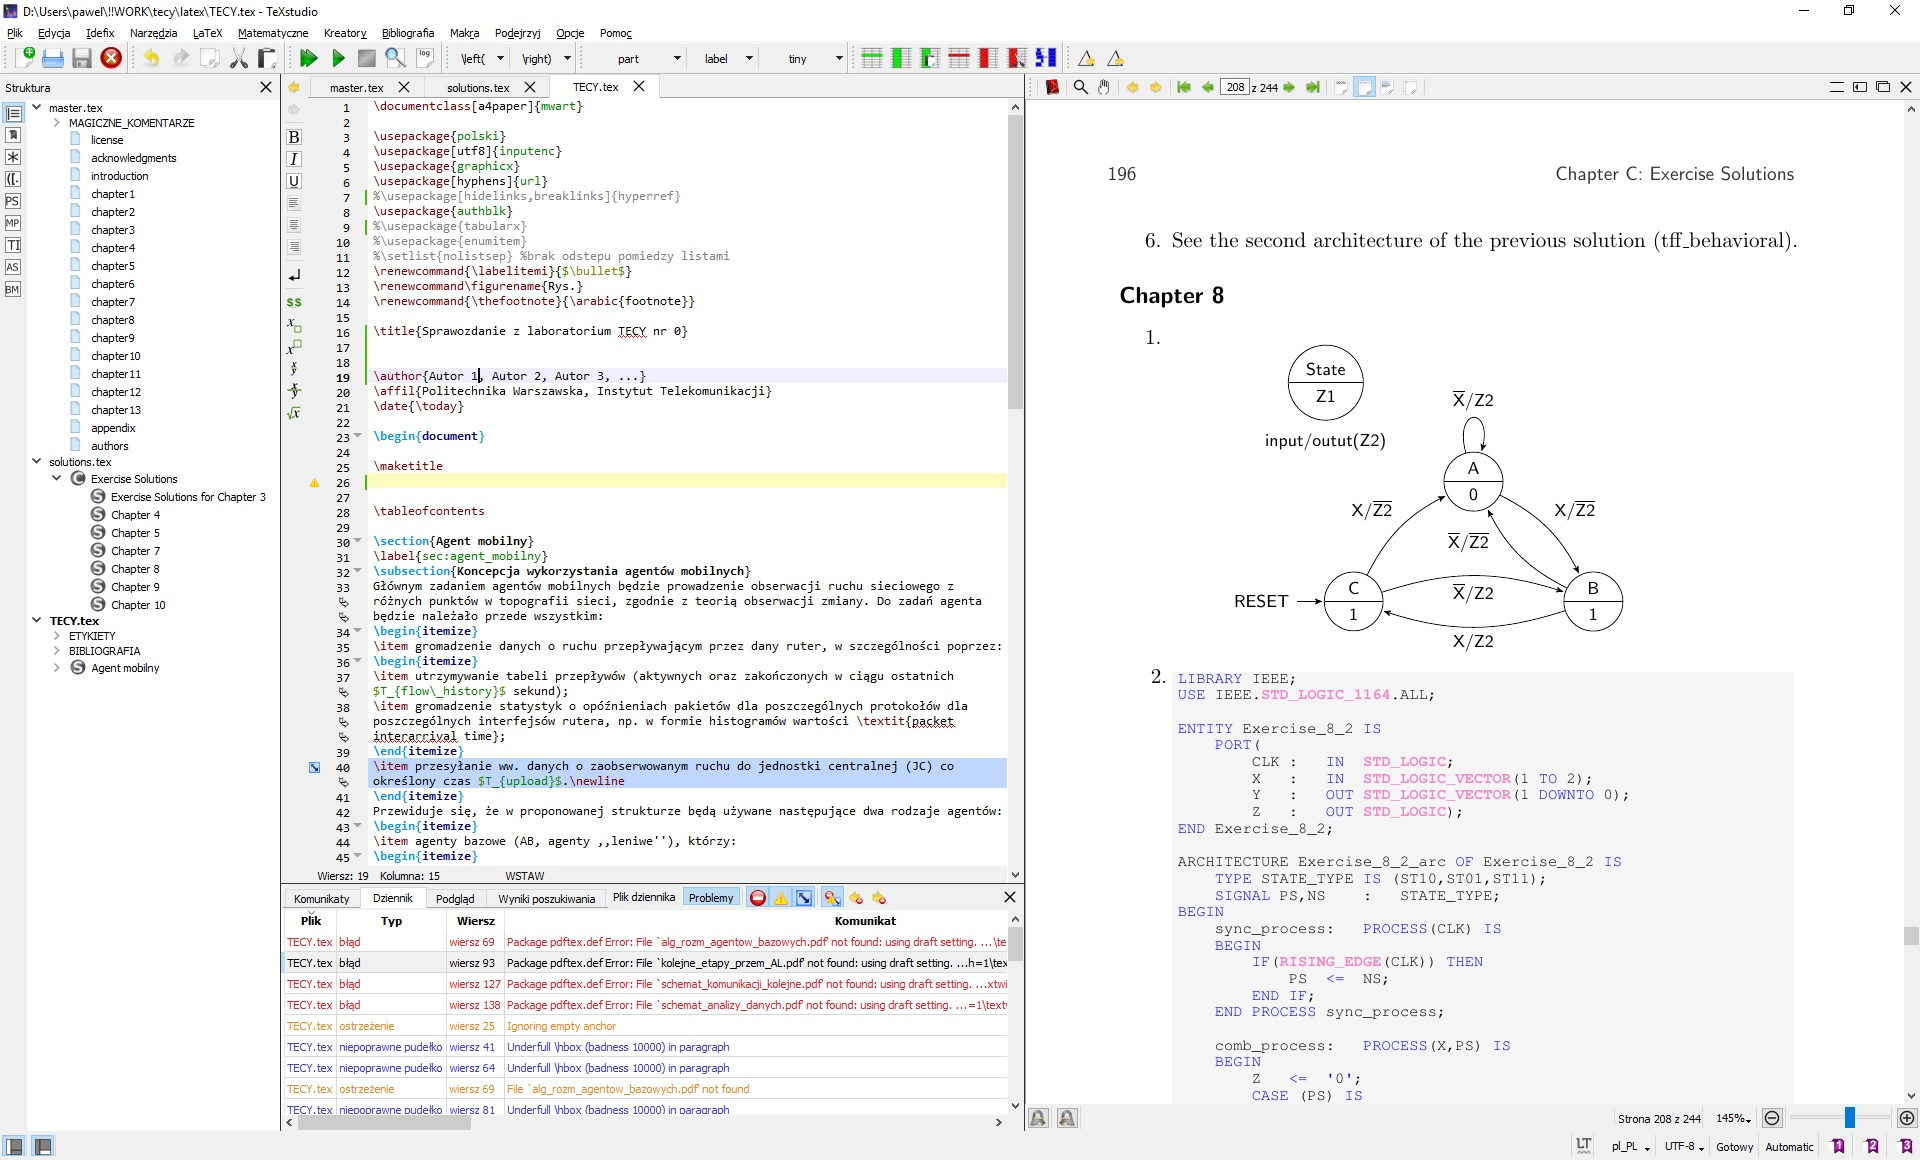
\includegraphics[width=0.5\textwidth]{rysunek_1.jpg}
\caption{\label{fig:rysunek_1}Widok edytora TeXstudio \cite{TeXstudio}}
\end{figure}
\FloatBarrier %zatrzymanie przenoszenia rysunku

\subsection{Tablice}
\begin{table}[h]
	\begin{center}
\caption{Przykładowa tabela}
\label{tab:tabela_przyklad}
\begin{tabular}{|r|l|c|c|}
	\hline 
	Miejsce & Drużyna & Gole & Punkty \\
	\hline \hline
	1 & Legia & 12 & 36 \\
	2 & Górnik & 10 & 30 \\
	3 & Widzew & 8 & 24\\
	4 & ŁKS & 7 & 21 \\ \hline
\end{tabular}
\end{center}
\end{table}
\FloatBarrier %zatrzymanie przenoszenia rysunku

\subsection{Wydruki}
\begin{lstlisting}[label=lst:wydruk,caption={Testowy program w Verilog},language=Verilog,numbers=left]
module lfsr_4 //rejestr o dlugosci 4
#(parameter n=4)
(
  input clk,
  input a_reset,
  input load,
  input [n-1:0]  a,
  output [n-1:0] result
);

reg [n-1:0] register;

always@(posedge clk, posedge a_reset)
if(a_reset)
  register <= 0;
else 
  if(load)
   register <= 1; // inicjacja
  else
   register <= {register[0],register[3:2], register[1]^register[0]};

assign result = register;

endmodule
\end{lstlisting}

\subsection{Matematyka}
Przykład użycia trybu matematycznego (poniżej).

The mass-energy equivalence is described by the famous equation

$$E=mc^2$$ %wysrodkowany bez numeracji

discovered in 1905 by Albert Einstein. 
In natural units ($c$ = 1), the formula expresses the identity %w tekscie

\begin{equation} %wysrodkowany z numeracja
E=m
\end{equation}

\subsection{Oprogramowanie - wersja Windows}
\label{sec:oprogramowanie}
Do pracy w środowisku \LaTeXe{} (wersja aktualnie używana) proponuję (wybór subiektywny i~jedynie słuszny) następujący zestaw oprogramowania \cite{Ghostscript, MikTeX, TeXstudio}, instalacja w takiej kolejności:
\begin{itemize}
\item Ghostscript -- interpreter plików PostScript i PDF  \url{https://www.ghostscript.com/},
\item MikTeX -- dystrybucja dla Windows  \url{https://miktex.org/} - zestaw narzędzi,
\item Adobe Reader -- przeglądarka plików PDF \url{https://acrobat.adobe.com/pl/pl/},
\item TeXstudio -- edytor i kompilator \url{https://texstudio.org/},
\item (opcjonalnie) Słownik PL do edytora -- należy zaimportować w edytorze (rys. \ref{fig:rysunek_spr})  \url{https://extensions.openoffice.org/en/project/polish-dictionary-pack},
\item (opcjonalnie) Java JRE (do uruchomienia LT) \url{https://www.java.com/pl/download/},
\item (opcjonalnie) Narzędzie Language Tool -- można uruchomić \textit{off-line} w edytorze \url{https://languagetool.org/download/LanguageTool-4.6.zip},
\end{itemize}

\begin{figure}[h]
	\centering
	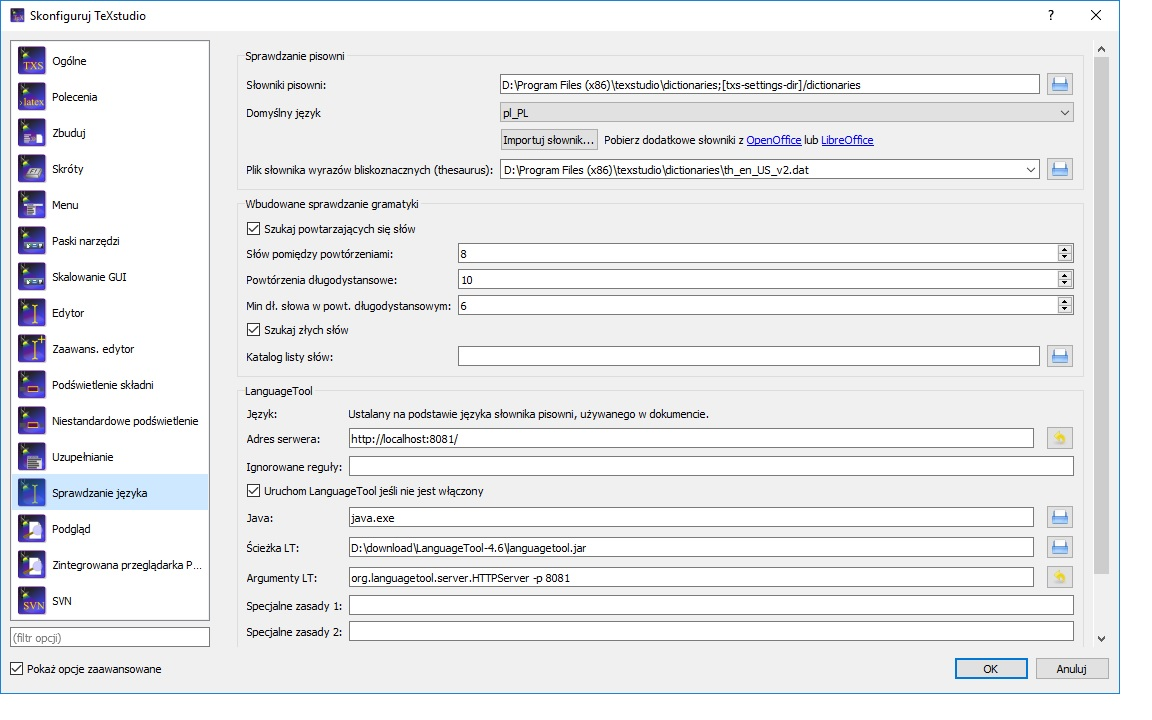
\includegraphics[width=1\textwidth]{texstudio_sprawdzanie_jezyka.jpg}
	\caption{\label{fig:rysunek_spr}Widok edytora TeXstudio -- ustawianie opcji do sprawdzania języka}
\end{figure}

Jeżeli kompilacja pierwszego dokumentu nie przebiegnie prawidłowo, tzn. kompilator nie znajdzie czcionek, należy uruchomić program \texttt{updmap.exe} z~pakietu MikTex.

Dla zawansowanych: sposób na automatyczne dodawanie tabulatora po literach a, i, o, u,w, z aby nie zostawały na końcu linii -- sierotki. Wyzwalacz \textit{trigger} ma postać \begin{verbatim}
(?language:latex)\sa\s|\si\s|\so\s|\su\s|\sw\s|\sz\s
\end{verbatim}

\begin{figure}[h]
	\centering
	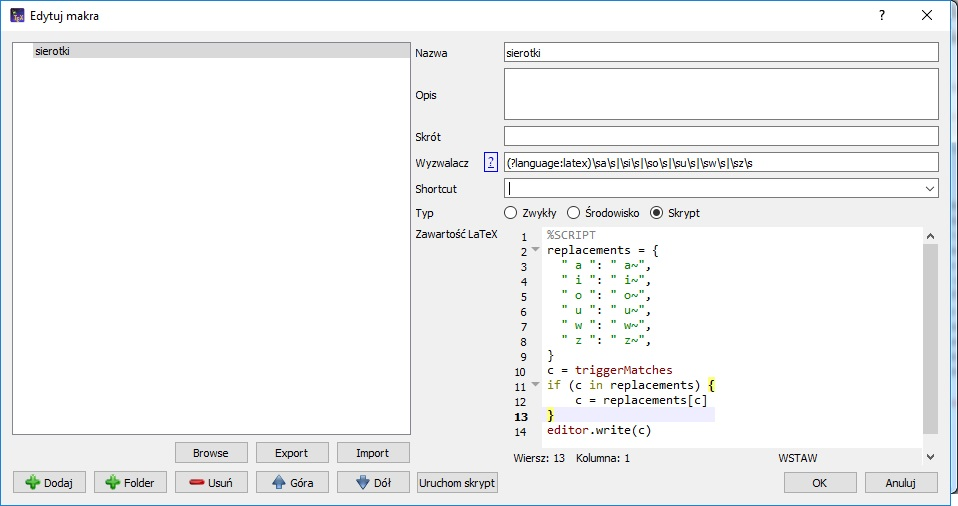
\includegraphics[width=1\textwidth]{sierotki.jpg}
	\caption{\label{fig:sierotki}Widok edytora TeXstudio -- makro dla sierotek}
\end{figure}

\begin{lstlisting}[label=lst:sierotki,caption={Widok edytora TeXstudio -- dodanie makra do sierotek},numbers=left]
%SCRIPT
replacements = {
" a ": " a~",
" i ": " i~",
" o ": " o~",
" u ": " u~",
" w ": " w~",
" z ": " z~",
}
c = triggerMatches
if (c in replacements) {
c = replacements[c]
}
editor.write(c)
\end{lstlisting}


\subsection{Inne strony}
\begin{itemize}
\item Obowiązkowa lektura: \url{ftp://ftp.gust.org.pl/TeX/info/lshort/polish/lshort2e.pdf}	
\item \url{http://www.mif.pg.gda.pl/homepages/sylas/students/wdi/index.html},
\item \url{https://www.mimuw.edu.pl/~mbodnar/prosem/wprowadzenie_v2016.pdf}	
\item \url{http://latex-kurs.x25.pl//}
\item \url{https://matematyka.pl/viewtopic.php?t=28951}	
\item \url{https://pl.wikibooks.org/wiki/LaTeX}	
\item \url{https://en.wikibooks.org/wiki/LaTeX}
\item Edytor i kompilator \textit{on-line} Overleaf -- także do pracy grupowej \url{https://www.overleaf.com/}
\item \url{https://www.google.com/search?q=latex+tutorial+pl} \dots	
\end{itemize}
 % każdy rozdział w osobnym pliku. 

%\newpage % Zaleca się otwieranie rozdziału od nowej strony
%\section{Summatio}      % Ale można też pisać w jednym. 
%\kant[5-6]

%--------------------------------------------
% Literatura
%--------------------------------------------
\newpage
\printbibliography
%--------------------------------------------
% Spisy (opcjonalne)
%--------------------------------------------
\newpage

% Wykaz symboli i skrótów.
% Pamiętaj, żeby posortować symbole alfabetycznie
% we własnym zakresie. Ponieważ mało kto używa takiego wykazu, 
% uznałem, że robienie automatycznie sortowanej listy
% na poziomie LaTeXa to za duży overkill. 
% Makro \acronymlist generuje właściwy tytuł sekcji, 
% w zależności od języka.
% Makro \acronym dodaje skrót/symbol to listy, 
% zapewniając podstawowe formatowanie.
% //AB
\vspace{0.8cm}
\acronymlist
\acronym{EiTI}{Wydział Elektroniki i Technik Informacyjnych}
\acronym{PW}{Politechnika Warszawska}
\acronym{FPGA}{Field Programmable Gates Array}
\acronym{DLP}{Discrete Logarithm Problem}
\acronym{GF}{Galois Field (ciało skończone)}

\listoffigures              % Spis obrazków. 
\vspace{1cm}                % vertical space
\listoftables               % Spis tabel. 
\vspace{1cm}               % vertical space
\lstlistoflistings 		% Spis wydruków
\vspace{1cm}                % vertical space
\listofappendices           % Spis załączników

% Załączniki

%\newpage
%\appendix{Nazwa załącznika 1}
%\lipsum[1]
%
%\newpage
%\appendix{Nazwa załącznika 2}
%\lipsum[1]
% Załączniki

%\newpage

% jesli sa w~Zalacznikach tabele, rysunki, tak na szybko.. i~wylaczyc \listofappendices
%\section*{Załącznik I. Wykaz komend AT czujnika parkowania AN-101D firmy Shenzhen Winext Technology}
%%\appendix{Wykaz komend AT czujnika parkowania AN-101D firmy Shenzhen Winext Technology.}
%\setcounter{section}{1}
%\renewcommand\thetable{I.\arabic{table}}
%\input{tex/zal-1-komendy-at}
%
%\newpage
%\section*{Załącznik II. Ramki komunikacyjne czujnika parkowania AN-101D firmy Shenzhen Winext Technology}
%%\appendix{Ramki komunikacyjne czujnika parkowania AN-101D firmy Shenzhen Winext Technology.}
%\renewcommand\thefigure{II.\arabic{figure}}
%\input{tex/zal-2-ramki-komunikacyjne}




\end{document} % Dobranoc. 

